\documentclass[a4paper,11pt]{article}
\usepackage{amsmath}
\usepackage[frenchb]{babel}
\usepackage[utf8]{inputenc}
\usepackage{fontspec} 
\usepackage[T1]{fontenc}
\usepackage{amssymb}
\title{Université d'été - Rapport}
\author{Ibanez Thomas, Lovino Maxime, Tournier Vincent}
\begin{document}
\maketitle
\section{Introduction}
WaspRunner est un projet miniature et compact de traceur GPS pour joggeurs soucieux de travailler leur VMA.\newline
WaspRunner se compose de trois éléments : un module traceur à emporter avec soi durant la course (fort heureusement le module est léger et compact - il peut facilement être transporté dans une valise à roulette), un serveur web sur Raspberry Pi, ainsi que d'une application Android.\newline
Le traceur est lui-même fait d'une carte waspmote équipée d'un module GPS et GPRS, d'une carte wifi dont la simplicité n'a d'égal que la fiabilité, d'une batterie faisant aussi office de lest pour que le coureur ne dépasse pas les limitations de vitesses du code de la route, ainsi que d'une carte microSD pour sauvegarder les courses.\newline
Le serveur web récupère les données GPS du traceur, les traite et les stocke. Il fournit également la possibilité de consulter les rapports de courses sur Internet.\newline
L'application Android permet quant à elle de recevoir les rapports de course directement sur son smartphone.\newline
\section{Réalisation}
\subsection{Base de données}
La base de données se présente selon le schéma suivant: \newline
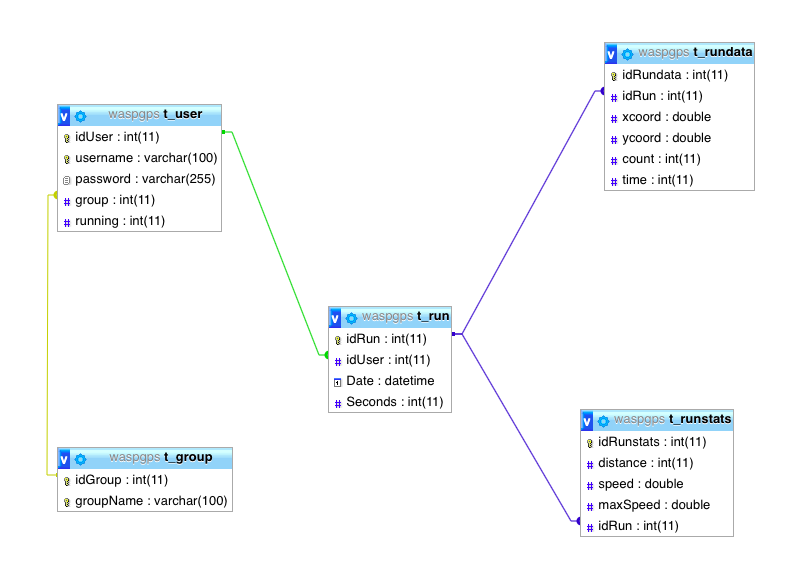
\includegraphics[scale=0.4]{db.png}
\subsection{Récupération et envoi des données GPS}
La première étape pour notre application est de récupérer la position actuelle via GPS, le module GPRS+GPS de la Waspmote s'occupe de nous donner la position en degrés [-180;180].\newline
Nous appliquons ensuite un code correcteur d'erreurs afin d'éviter qu'un problème de communication n'entraine l'insertion de fausses données dans la course.\newline
Une fois la position définie, la waspmote, si une carte SIM et une connexion sont disponible, va envoyer une requête GET sur l'application web (page run.php), en définissant des flags dans l'url qui seront interprétés par le code php.
\begin{itemize}
\item uid: l'identifiant de l'utilisateur courant, (par défaut 1)
\item start: doit être défini en cas de début de course
\item x: longitude (en degrés)
\item y: latitude (en degrés)
\item cnt: numéro du point envoyé
\item time: temps (en seconde) écoulé depuis le début de la course
\item end: envoyé en fin de course
\end{itemize}
Voici un exemple de communication entre la waspmote et l'application web
\begin{itemize}
\item /run.php?uid=1\&start
\item /run.php?uid=1\&x=<longitude>\&y=<latitude>\&time=12\&cnt=1
\item /run.php?uid=1\&x=<longitude>\&y=<latitude>\&time=18\&cnt=2
\item /run.php?uid=1\&x=<longitude>\&y=<latitude>\&time=23\&cnt=3
\item \ldots
\item /run.php?uid=1\&time=2704\&end
\end{itemize}

\subsection{Traitement des données}
L'application web s'occupe du lien avec la base de données, au départ de la course un fannion running dans la ligne de l'utilisateur est défini à l'id de la course en cours.\newline
Ensuite à chaque fois qu'un point est envoyé, données du point (x,y,cnt et time) sont ajoutés dans la table t\_rundata.\newline
Lorsque l'application reçoit le fannion end, la case running de l'utilisateur est remise à 0 et les statistiques de course sont calculées.
Le calcul de la distance au sol est fait par la formule d'Haversine.
\begin{equation*}
a = sin^2(\frac{\varphi_1 - \varphi_2}{2}) + cos(\varphi_1) * cos(\varphi_2) * sin^2(\frac{\lambda_1 - \lambda_2}{2})
\end{equation*}
\begin{equation*}
d = 2r *arctan\left(\frac{\sqrt{a}}{\sqrt{1-a}}\right)
\end{equation*}
Où \newline
$\varphi_1 \; et \; \varphi_2$ sont les longitudes des deux points\newline
$\lambda_1 \; et \; \lambda_2$ sont les latitudes des deux points\newline
$r$ est le rayon de la terre (6371 Km)\newline
\subsection{Stockage des données en cas de problème de réseau}
Dans le cas où le module est incapable, pour une raison ou une autre, de se connecter au réseau GPRS avant qu'une course ne soit démarrée, il nous a fallu trouver un moyen de ne pas rendre le module inutilisable. Pour cela, nous avons fait le choix de permettre à l'utilisateur de sauvegarder les données de la course sur une carte SD.\newline
Dans le cas où le réseau GPRS est inaccessible au moment où doit démarrer une course, les données GPS et tous les points sont sauvegardés sur un fichier texte présent dans la carte SD, sous la forme de lignes de commandes. La course se déroule alors normalement, chaque point étant sauvegardé sur la carte SD.\newline
Lorsque la course est stoppée, le fichier est rendu disponible à l'envoi. Immédiatement, la carte WiFly s'active et essaye de se connecter au réseau WiFi sauvegardé dans sa configuration. De la même manière, si la carte s'allume et qu'un fichier de course est présent en mémoire, elle essayera d'abord d'envoyer le fichier avant de laisser l'utilisateur démarrer une course.\newline
Sitôt que la carte parvient à se connecter à un réseau WiFy, elle ouvre une connexion vers un socket java présent sur le serveau web. Lorsque la connexion TCP est établie, la carte envoie ligne par ligne les données présentes sur le fichier, puis se déconnecte et, si les données ont été correctement envoyée, détruit le fichier. Une nouvelle course peut alors être lancée.\newline
Dans le cas où la carte est incapable d'obtenir une connexion WiFi ou TCP, et ce afin d'éviter un comportement bloquant pour l'utilisateur, un timeout a été mis en place. Globalement, une tentative de connexion prend 5 secondes, aussi nous avons limité le nombre de tentatives à 12 afin que la carte essaye de se connecter pendant environ une minute avant d'abandonner et de laisser l'utilisateur démarrer, s'il le souhaite, une nouvelle course. Par ailleurs, si cette nouvelle course doit être enregistrée sur la carte SD, elle sera simplement ajoutée à la suite de celle déjà présente.\newline
\subsection{Application Android}
Une application Android a également été réalisée, il s'agit de WaspDroid.
\subsubsection{Recupération des données et stockage}
Pour récupérer les données de course depuis le serveur, un hook php dédié a été mis en place, en effet: \newline
\verb+/android.php?uid=1&listrun+ \newline
permet de récupérer la liste des courses dans un format CSV de la forme \verb+runID;date;temps+. Ensuite, nous pouvons utiliser \newline
\verb+/android.php?uid=1&rundata&idRun=X+ \newline
pour récupérer la liste des points pour la course X. Ses données sont en CSV de la forme
\verb+x;y;count;temps+ \\

Les données sont stockées dans une base de données locale SQLite qui sert de cache en cas de perte de connexion de l'appareil et permet de rendre l'application plus rapidement fonctionnelle, étant donnée que les données sont déjà chargées sont devoir envoyer des requêtes au serveur. Les classes \verb+RunDBContract+ et \verb+RunDBHelper+ s'occupent de cette base de données. La classe \verb+PHPConnector+ prend en charge l'intéraction avec notre serveur, elle hérite de \verb+AsyncTask+ pour lui permettre de charger les données dans un thread séparé. (obligatoire sur Android)\\

Dans les réglages de l'application, il est possible de définir l'URL et le port du serveur à utiliser (par défaut sampang.internet-box.ch et port 8080) ainsi que de remettre à zéro la base de données de cache.

\subsubsection{Interface graphique et API Maps}
L'interface graphique de l'application est assez simple, nous avons deux activités principales. \verb+MainActivity+ qui affiche la liste des différentes courses et qui lance \verb+DetailView+ lorsqu'on clique sur l'une d'entre elles. \\

Dans la vue détaillée, nous affichons les différentes statistiques de la course, ainsi qu'un fragment Google Maps avec le parcours de celle-ci. L'application demande la permission à l'utilisateur à ce moment-là pour utiliser sa localisation et pouvoir l'afficher sur la carte également.

\end{document}
